\documentclass[12pt, titlepage]{article}

\usepackage{fullpage}
\usepackage[round]{natbib}
\usepackage{multirow}
\usepackage{booktabs}
\usepackage{tabularx}
\usepackage{graphicx}
\usepackage{float}
\usepackage{hyperref}
\hypersetup{
    colorlinks,
    citecolor=blue,
    filecolor=black,
    linkcolor=red,
    urlcolor=blue
}

%% Comments

\usepackage{color}

\newif\ifcomments\commentstrue %displays comments
%\newif\ifcomments\commentsfalse %so that comments do not display

\ifcomments
\newcommand{\authornote}[3]{\textcolor{#1}{[#3 ---#2]}}
\newcommand{\todo}[1]{\textcolor{red}{[TODO: #1]}}
\else
\newcommand{\authornote}[3]{}
\newcommand{\todo}[1]{}
\fi

\newcommand{\wss}[1]{\authornote{blue}{SS}{#1}} 
\newcommand{\plt}[1]{\authornote{magenta}{TPLT}{#1}} %For explanation of the template
\newcommand{\an}[1]{\authornote{cyan}{Author}{#1}}

%% Common Parts

\newcommand{\progname}{Scanalyze AI} % PUT YOUR PROGRAM NAME HERE
\newcommand{\authname}{Team 16, Ace
\\ Hamza Issa
\\ Ahmad Hamadi
\\ Jared Paul
\\ Gurnoor Bal} % AUTHOR NAMES                  

\usepackage{hyperref}
    \hypersetup{colorlinks=true, linkcolor=blue, citecolor=blue, filecolor=blue,
                urlcolor=blue, unicode=false}
    \urlstyle{same}
                                


\newcounter{acnum}
\newcommand{\actheacnum}{AC\theacnum}
\newcommand{\acref}[1]{AC\ref{#1}}

\newcounter{ucnum}
\newcommand{\uctheucnum}{UC\theucnum}
\newcommand{\uref}[1]{UC\ref{#1}}

\newcounter{mnum}
\newcommand{\mthemnum}{M\themnum}
\newcommand{\mref}[1]{M\ref{#1}}

\begin{document}

\title{Module Guide for \progname} 
\author{Team 16, Ace\\
Hamza Issa \\
Ahmad Hamadi \\
Jared Paul \\
Gurnoor Bal}
\date{January 18, 2025}

\maketitle

\pagenumbering{roman}

\section{Revision History}

\begin{tabularx}{\textwidth}{p{3cm}p{2cm}X}
\toprule
{\bf Date} & {\bf Version} & {\bf Notes}\\
\midrule
January 6, 2025 & 1.0 & Initial draft of the Module Guide (MG) document created.\\
January 8, 2025 & 1.1 & Added module descriptions and dependencies. Updated section on module interactions.\\
January 10, 2025 & 1.2 & Incorporated feedback from team review. Clarified module responsibilities and refined explanations.\\
January 12, 2025 & 1.3 & Improved formatting and consistency with the MIS document. Adjusted terminology for clarity.\\
January 14, 2025 & 1.4 & Revised diagrams and module relationships. Added missing assumptions and constraints.\\
January 16, 2025 & 1.5 & Finalized the document. Ensured alignment with project requirements and other documents (MIS, SRS).\\
March 29, 2025 & 2.0 & Final refinements to align the modules more closely with our finalized codebase and product.\\
April 4, 2025 & 3.0 & Finalized the document. Ensured alignment with project requirements and other documents (MIS, SRS) and addressed feedback.\\
\bottomrule
\end{tabularx}

\newpage

\section{Reference Material}

This section records information for easy reference.

\subsection{Abbreviations and Acronyms}

\renewcommand{\arraystretch}{1.2}
\begin{tabular}{l l} 
  \toprule		
  \textbf{symbol} & \textbf{description}\\
  \midrule 
  AC & Anticipated Change\\
  DAG & Directed Acyclic Graph \\
  M & Module \\
  MG & Module Guide \\
  OS & Operating System \\
  R & Requirement\\
  SC & Scientific Computing \\
  SRS & Software Requirements Specification\\
  Chest Scan & Explanation of program name\\
  UC & Unlikely Change \\
  \bottomrule
\end{tabular}\\

\newpage

\tableofcontents

\newpage

\pagenumbering{arabic}

\section{Summary of Changes Made to the MG}

\begin{itemize}
    \item The Module Decomposition section was rewritten to reflect the revisions to the modules as shown in the MIS document. This change is a direct result of our change from a diffusion model-based project to a multi-class classification ML model.
    \item The Model Hierarchy and mapping sections were likewise changed to reflect the new project direction.
    \item In these sections, we compiled the new modules required for this project and detailed their relevant mappings to other modules as well as its respective hierarchy.
    \item As the project had this change in direction, moving to the multiclassification route, the anticipated changes were updated to describe potential changes that could occur given the new modules and project direction.
\end{itemize}

\section{Introduction}

To build software systems that are reliable, easy to maintain, and adaptable to future changes, it's important to break them down into smaller, manageable parts. This approach, known as modular design, ensures that each part of the system has a single responsibility and can be developed, tested, and updated independently of the others.

This document outlines the structure of a modular system designed to support a machine learning model that performs multi-disease classification on chest X-ray images. The goal of this system is to take raw medical image data, prepare it for training, define a suitable neural network architecture, train the model using the prepared data, and then make the model accessible through a backend and user interface.

Each module in the system was created with the idea that it should hide its internal details (or "secrets") from other parts of the system. By doing this, the system becomes easier to understand and modify - for example, if we want to improve the model architecture or adjust how the data is preprocessed, we can do so without affecting unrelated parts of the project.

This document is intended to explain how the system is organized and how the modules interact. It is meant to help:

\begin{itemize}
    \item \textbf{New developers} understand the system and get up to speed quickly
    \item \textbf{Future contributors} make changes without accidentally breaking things
    \item \textbf{Reviewers or instructors} verify that the design meets the project goals
\end{itemize}

This design document aims to provide a structured and abstract explanation of the larger software architecture of this project. As a result, this document will include the large system design, single responsibility modules and the relationships between them. The object is to ensure that future stakeholders and engineers can easily digest the architecture presented such that they may become capable to contribute to the project if necessary.

\newpage

\section{Anticipated and Unlikely Changes}

Anticipated changes are the areas of the system that are most likely to evolve and have been designed to accommodate future adjustments. These changes are encapsulated within specific modules to ensure the system's flexibility.

\subsection{Anticipated Changes}

\begin{itemize}
    \item \textbf{AC1: Model Architecture Upgrades} \\
    As new multi-disease classification models are published or transfer learning methods improve, the current CNN model may need to be updated or replaced. The system's modular architecture ensures that the model definition and training pipeline can be swapped or extended without major changes to the rest of the codebase.
    
    \item \textbf{AC2: Dataset Expansion and Variation} \\
    The system currently uses the NIH Chest X-ray dataset. In the future, new datasets (e.g., CheXpert, MIMIC-CXR) may be added to improve performance or generalization. The DataRetrieval and DataPreparation modules are designed to accommodate multiple datasets and make it easy to plug in additional sources with minimal code changes.
    
    \item \textbf{AC3: Frontend Feature Enhancements} \\
    User-facing features such as more detailed result visualizations (e.g., confidence scores, heatmaps), improved PDF exports, or interactive diagnosis explanations may be added. These changes would primarily affect the ModelInterface module without requiring changes to the backend or model logic.
    
    \item \textbf{AC4: User Authentication and Role Management} \\
    As the system evolves, there may be a need to introduce more complex user roles (e.g., admin, medical reviewer, student) or integrate external authentication systems (e.g., hospital SSO or OAuth). These changes would be localized within the AuthClient and Authorization modules.
    
    \item \textbf{AC5: Model Performance Evaluation and Monitoring} \\
    New evaluation metrics, dashboards, or logging mechanisms may be introduced to better track model performance over time. These additions would help provide greater insight into how the model performs across different datasets, classes, and use cases.
    
    \item \textbf{AC6: Integration with External Services} \\
    In the future, the system may be required to integrate with third-party tools, such as electronic medical record systems, hospital databases, or cloud-based ML services. The modular backend and controller logic (MLBackend, Config) are prepared to support such integrations with minimal disruption.
\end{itemize}

\newpage

\subsection{Unlikely Changes}

Unlikely changes refer to parts of the system architecture that are not expected to require modification under typical usage or foreseeable project evolution. These areas have been designed with long-term stability in mind and are either foundational to the system's operation or tightly coupled to domain-specific constraints.

\begin{itemize}
    \item \textbf{UC1: Abandoning the Modular Architecture Design} \\
    The project is built around modularity and separation of concerns as core software engineering principles. Switching to a monolithic or less modular architecture would compromise maintainability and scalability. It is unlikely that this approach would be reconsidered unless the entire project is restructured, which contradicts its maintainability goals.
    
    \item \textbf{UC2: Removal of Machine Learning Components} \\
    Since the core purpose of this project is multi-disease classification using machine learning, the removal of ML-related components such as ModelArchitecture, Training, or MLBackend would fundamentally alter the system's purpose. These components are central to the system and are not expected to be deprecated.
    
    \item \textbf{UC3: Eliminating User Authentication} \\
    User authentication through modules like AuthClient and Authorization provides a necessary security layer for medical applications, especially in regulated environments. Removing authentication entirely is highly improbable, as it would expose the system to privacy and compliance risks, especially when deployed in real-world or clinical settings.
    
    \item \textbf{UC4: Switching Away from Medical Imaging} \\
    The project is domain-specific to chest X-ray analysis, and every module - from data preparation to visualization - is aligned with this domain. A pivot to a completely different domain (e.g., non-medical computer vision tasks) would render large parts of the architecture obsolete and is not aligned with the system's design objectives.
    
    \item \textbf{UC5: Replacing All Dataset Sources with Synthetic Data} \\
    Although synthetic datasets may be used for augmentation or research, replacing all real-world datasets like NIH Chest X-rays with synthetic data would limit clinical relevance and model generalizability. Therefore, it is unlikely that synthetic data would become the sole source for training and evaluation.
    
    \item \textbf{UC6: Discontinuation of User Interface} \\
    The ModelInterface module provides crucial access to model predictions and results for users, whether they are clinicians, researchers, or students. Eliminating the UI layer in favor of purely API-based access would reduce usability and is not aligned with the system's goal of providing a user-friendly diagnostic tool.
\end{itemize}

\section{Module Hierarchy} \label{SecMH}
This section of the document describes the modules that make up the project and their related hierarchy. Table~\ref{TblEncapsulation} categorizes the modules based on encapsulation, whereas Table~\ref{TblMVC} categorizes modules according to the MVC architecture. Each category can be identified as nodes in a tree, where each of the respective modules in each category are leaves of that node.

Total Module List:

\begin{itemize}
    \item M1: ModelInterface
    \item M2: AuthClient
    \item M3: DataRetrieval
    \item M4: DataPreparation
    \item M5: Authorization
    \item M6: Config
    \item M7: MLBackend
    \item M8: ModelArchitecture
    \item M9: Training
\end{itemize}

\begin{table}[h!]
\centering
\begin{tabular}{|p{0.3\textwidth}|p{0.6\textwidth}|}
\hline
\textbf{Node} & \textbf{Leaf} \\
\hline
\textbf{Hardware Encapsulation} & N/A \\
\hline
\textbf{Behaviour Encapsulation} & ModelInterface, AuthClient, DataRetrieval, DataPreparation, Authorization \\
\hline
\textbf{Software Decision Encapsulation} & Config, MLBackend, ModelArchitecture, Training \\
\hline
\end{tabular}
\caption{Encapsulation}
\label{TblEncapsulation}
\end{table}

\textbf{Table 2: Model-View-Controller (MVC)}
\begin{table}[h!]
\centering
\begin{tabular}{|l|l|}
\hline
\textbf{Node} & \textbf{Leaf} \\
\hline
\textbf{Model Module} & DataRetrieval, DataPreparation, ModelArchitecture, Training \\
\hline
\textbf{View Module} & ModelInterface, AuthClient \\
\hline
\textbf{Controller Module} & Config, MLBackend, Authorization \\
\hline
\end{tabular}
\caption{Model-View-Controller}
\label{TblMVC}
\end{table}

\newpage

\section{Connection Between Requirements and Design} \label{SecConnection}
The design of the system is intended to satisfy the requirements developed in the SRS. In this stage, the system is decomposed into modules. The connection between requirements and modules is listed in Table~\ref{TblRT}.

\begin{table}[h!]
\centering
\begin{tabular}{|l|l|}
\hline
\textbf{Req.} & \textbf{Modules} \\
\hline
R1 & M9, M3, M5 \\
R2 & M4, M5 \\
R3 & M1, M2 \\
R4 & M7, M9 \\
R5 & M6, M5 \\
R6 & M3, M9 \\
R7 & M1, M8 \\
\hline
\end{tabular}
\caption{Trace Between Requirements and Modules}
\label{TblRT}
\end{table}


\section{Module Decomposition}

The structure of the system follows modular design principles, where each module encapsulates a specific "secret" or design decision. Below are the detailed descriptions of the modules:

\subsection{AuthClient Module (M2)}

\textbf{Secrets:} Manages user identity, authentication, and access control. Ensures only verified users can interact with model features by handling login, registration, and token-based session management.

\textbf{Services:} Authenticates users via login and registration forms, stores JWT tokens securely in browser storage, attaches authorization headers to API requests, and handles logout and token expiration gracefully via interceptors.

\textbf{Implemented By:} Login.tsx, Register.tsx, api.ts

\textbf{Type of Module:} Record, Library

\subsection{DataRetrieval Module (M3)}

\textbf{Secrets:} Handles the automated download and extraction of the NIH Chest X-ray image dataset. Abstracts away the raw data acquisition process to ensure that downstream data preparation modules always operate on a consistent and expected file structure.

\textbf{Services:} 
\begin{itemize}
    \item Downloads chest X-ray image archives from specified NIH URLs if they are not already present.
    \item Extracts .tar.gz image files into the ./data/images directory.
    \item Ensures idempotency by checking for existing files before downloading.
    \item Supports batch retrieval and consistent folder organization for preprocessing modules.
\end{itemize}

\textbf{Implemented By:} train.py

\textbf{Type of Module:} Utility, Function Library

\subsection{DataPreparation Module (M4)}

\textbf{Secrets:} Processes and prepares the NIH Chest X-ray dataset for training and evaluation. Handles CSV parsing, label binarization, dataset filtering, stratified data splitting, transformation pipeline creation, and statistical analysis required for multi-label classification.

\textbf{Services:} 
\begin{itemize}
    \item Loads and parses the Data\_Entry\_2017.csv metadata file.
    \item Cleans and filters records (e.g., removes "No Finding", optionally trims rare classes).
    \item Converts multi-label disease strings into binary vectors for each class.
    \item Splits data into training and validation sets using stratified sampling.
    \item Creates image transformation pipelines with optional augmentations for training.
    \item Calculates class-wise positive weights and average label counts for loss balancing.
\end{itemize}

\textbf{Implemented By:} train.py

\textbf{Type of Module:} Function Library

\subsection{Authorization Module (M5)}

\textbf{Secrets:} Handles authentication and registration logic using secure password hashing and JWT-based authorization. Manages user identity, roles, and token validation to ensure secure access to protected resources.

\textbf{Services:} 
\begin{itemize}
    \item Provides REST APIs for user login and registration, generates and validates JWT tokens, manages user and role persistence, and injects authenticated users into the Spring Security context via filters.
\end{itemize}

\textbf{Implemented By:} 
\begin{itemize}
    \item AuthController.java
    \item AuthService.java, AuthServiceImpl.java
    \item JwtTokenProvider.java, JWTAuthenticationFilter.java
    \item CustomUserDetailsService.java
    \item User.java, Role.java, UserRepository.java, RoleRepository.java
\end{itemize}

\textbf{Type of Module:} Abstract Object, Record, Library

\section{Traceability Matrix}

The Traceability Matrix provides a mapping between the software requirements, anticipated changes, and the modules outlined in the design document. This ensures that each requirement and anticipated change is addressed by specific modules, fostering consistency, maintainability, and scalability.

\subsection{Traceability Between Requirements and Modules}

The table below maps the functional requirements (FR) from the Software Requirements Specification (SRS) to the corresponding modules responsible for their implementation:

\begin{table}[H]
\centering
\begin{tabular}{|l|l|}
\hline
\textbf{Requirement ID} & \textbf{Modules} \\ \hline
FR1 & M7 (MLBackend) \\ \hline
FR2 & M4 (DataPreparation) \\ \hline
FR3 & M8 (ModelArchitecture), M9 (Training) \\ \hline
FR4 & M1 (ModelInterface), M7 (MLBackend) \\ \hline
FR5 & M1 (ModelInterface) \\ \hline
FR6 & M1 (ModelInterface) \\ \hline
FR7 & M2 (AuthClient), M5 (Authorization) \\ \hline
FR8 & M5 (Authorization) \\ \hline
FR9 & M1 (ModelInterface), M7 (MLBackend) \\ \hline
FR10 & M1 (ModelInterface) \\ \hline
\end{tabular}
\caption{Traceability Between Requirements and Modules}
\label{TblFRM}
\end{table}

\subsubsection{Mapping Requirements to Modules}
Each functional requirement is addressed by one or more modules within the system:

\begin{itemize}
    \item \textbf{FR1:} Handled by the M7 (MLBackend) module to receive, validate, and forward image uploads in supported formats.
    \item \textbf{FR2:} Managed by the M4 (DataPreparation) module to preprocess uploaded images through resizing, normalization, and standardization.
    \item \textbf{FR3:} Supported by both the M8 (ModelArchitecture) and M9 (Training) modules to classify diseases and return predictions with confidence scores.
    \item \textbf{FR4:} Enabled by the M1 (ModelInterface) and M7 (MLBackend) modules to support multi-label disease classification and return multiple predictions per image.
    \item \textbf{FR5:} Delivered by the M1 (ModelInterface) module, which displays disease predictions, confidence scores, and visualization components in a readable format.
    \item \textbf{FR6:} Delivered by the M1 (ModelInterface) module, which allows users to download diagnostic reports containing predictions, heatmaps, and findings in a secure and accessible format.
    \item \textbf{FR7:} Implemented by the M2 (AuthClient) and M5 (Authorization) modules to authenticate users and enforce role-based access control across system features.
    \item \textbf{FR8:} Provided by the M5 (Authorization) module through a secure API interface for accepting image inputs and returning diagnostic results in JSON format.
    \item \textbf{FR9:} Managed by both the M1 (ModelInterface) and M7 (MLBackend) modules to detect and communicate input or system errors clearly to users.
    \item \textbf{FR10:} Delivered by the M1 (ModelInterface) module, which ensures that diagnostic details including prediction results, probabilities, and timestamps are clearly displayed to the user.
\end{itemize}

This mapping confirms that each functional requirement is appropriately addressed by one or more modules, reinforcing the system's alignment with its design goals and intended functionality.

\subsection{Traceability Between Anticipated Changes and Modules}

The table below identifies how anticipated changes (AC) outlined in the SRS and design document are addressed by specific modules, ensuring that the design is resilient to future updates:

\begin{table}[H]
\centering
\resizebox{\textwidth}{!}{
\begin{tabular}{|l|l|}
\hline
\textbf{Anticipated Change ID} & \textbf{Modules} \\ \hline
AC1: Model Architecture Upgrades & M8 (ModelArchitecture), M9 (Training) \\ \hline
AC2: Dataset Expansion and Variation & M3 (DataRetrieval), M4 (DataPreparation) \\ \hline
AC3: Frontend Feature Enhancements & M1 (ModelInterface), M2 (AuthClient) \\ \hline
AC4: User Authentication and Role Management & M2 (AuthClient), M5 (Authorization) \\ \hline
AC5: Model Performance Evaluation and Monitoring & M9 (Training) \\ \hline
AC6: Integration with External Services & M6 (Config), M7 (MLBackend), M5 (Authorization) \\ \hline
\end{tabular}
}
\caption{Traceability Between Anticipated Changes and Modules}
\label{TblACTM}
\end{table}

\subsubsection{Mapping Anticipated Changes to Modules}
Anticipated changes are encapsulated within specific modules to ensure that evolving requirements can be accommodated without disrupting the overall system:

\begin{itemize}
    \item \textbf{AC1:} ModelArchitecture and Training support improvements in model design, allowing for updated architectures and training strategies to be integrated easily.
    \item \textbf{AC2:} DataRetrieval and DataPreparation enable the system to handle new or expanded datasets through configurable loading, cleaning, and transformation pipelines.
    \item \textbf{AC3:} ModelInterface and AuthClient provide the user-facing components where new visual features and diagnostic feedback can be introduced.
    \item \textbf{AC4:} AuthClient and Authorization are responsible for login, registration, and user roles, supporting future changes in authentication methods or access levels.
    \item \textbf{AC5:} Training manages model evaluation logic and can be extended with new metrics, logging, and performance monitoring tools.
    \item \textbf{AC6:} Config, MLBackend, and Authorization facilitate backend configuration and external API access, supporting future integration with hospital systems or third-party services.
\end{itemize}

This mapping ensures that each anticipated change has been carefully considered in the design and is isolated to a small number of modules. This contributes to a more maintainable, scalable, and future-ready software architecture.

\newpage

\section{Use Hierarchy Between Modules}

\subsection{Model Modules}
\begin{table}[h!]
\centering
\begin{tabular}{|l|l|}
\hline
\textbf{Module} & \textbf{Uses} \\
\hline
DataRetrieval & None \\
\hline
DataPreparation & M3 (DataRetrieval) \\
\hline
ModelArchitecture & None \\
\hline
Training & M8 (ModelArchitecture), M4 (DataPreparation), M3 (DataRetrieval) \\
\hline
\end{tabular}
\caption{Model Modules}
\label{tab:model_modules}
\end{table}

\subsection{View Modules}
\begin{table}[h!]
\centering
\begin{tabular}{|l|l|}
\hline
\textbf{Module} & \textbf{Uses} \\
\hline
ModelInterface & MLBackend \\
\hline
AuthClient & Authorization \\
\hline
\end{tabular}
\caption{View Modules}
\label{tab:view_modules}
\end{table}

\subsection{Controller Modules}
\begin{table}[h!]
\centering
\begin{tabular}{|l|l|}
\hline
\textbf{Module} & \textbf{Uses} \\
\hline
MLBackend & DataRetrieval, DataPreparation, ModelArchitecture, Training \\
\hline
Authorization & AuthClient, Config \\
\hline
Config & None \\
\hline
\end{tabular}
\caption{Controller Modules}
\label{tab:controller_modules}
\end{table}

\subsection{Explanation of Use Hierarchy}
\begin{itemize}
    \item \textbf{Top-Down Structure:} The hierarchy starts with high-level view and controller modules, such as M1 (ModelInterface) and M7 (MLBackend), which coordinate system functionality and delegate responsibilities to underlying model modules.
    \item \textbf{Layered Dependency:} Each module depends on lower-level modules to provide specific functionality, following principles of modularity and separation of concerns. For example, M9 (Training) relies on M4 (DataPreparation), M8 (ModelArchitecture), and M3 (DataRetrieval) to train and evaluate the CNN model effectively.
    \item \textbf{Cross-Layer Interactions:} Controller modules like M7 (MLBackend) and M5 (Authorization) act as bridges between the frontend views (M1, M2) and the backend model logic. This allows the system to handle user input, manage access control, and invoke AI-based predictions seamlessly.
\end{itemize}



This use hierarchy supports a well-structured, modular design that promotes maintainability, testability, and ease of extension as the system evolves.

\begin{figure}[h!]
\centering
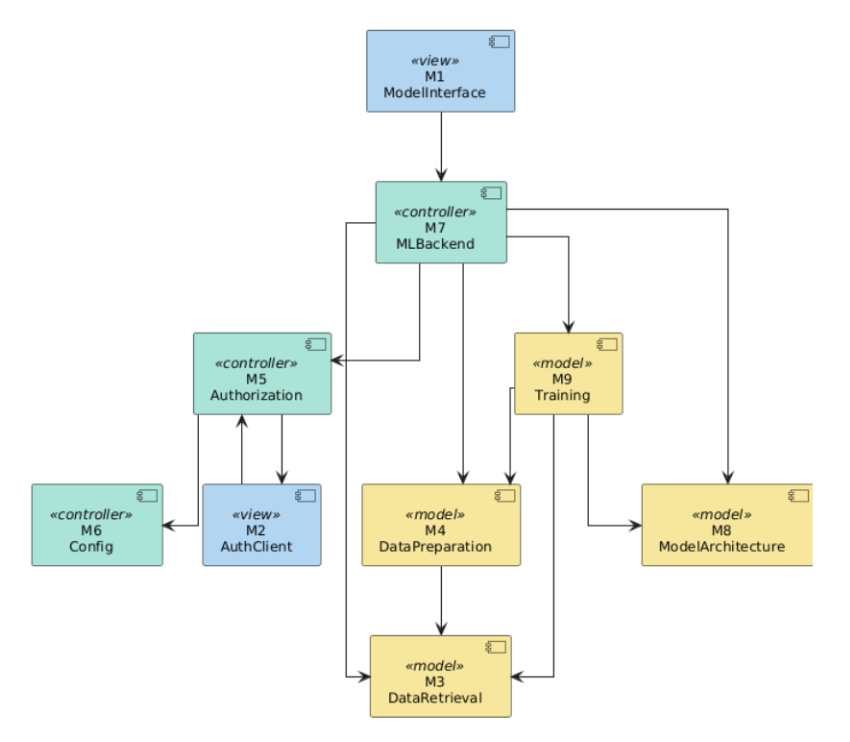
\includegraphics[width=\textwidth]{use_hierachy.png}
\caption{Use Hierarchy Between Modules}
\end{figure}

\section{User Interfaces}

Figma prototype includes \href{https://www.figma.com/proto/O3J164KiWA8uFswM7JgFy4/Capstone-Design?node-id=0-1&t=JT3KrFZiVb66Ch-1}{login page}, \href{https://www.figma.com/proto/O3J164KiWA8uFswM7JgFy4/Capstone-Design?node-id=0-1&t=JT3KrFZiVb66Ch-1}{main page} to upload an xray image, and the results of the uploaded image.

\section{Timeline}

\begin{table}[h!]
\centering
\begin{tabular}{|p{10cm}|l|}
\hline
\textbf{Task} & \textbf{Responsible Team Member(s)} \\
\hline
Define system architecture and module design (MG and MIS) & Entire Team \\
\hline
Develop data retrieval and preprocessing pipeline (CSV parsing, label binarization, transforms) & Harrison, Jared \\
\hline
Implement CNN model architecture and training logic & Jared, Ahmad \\
\hline
Design and implement model evaluation (metrics, accuracy tracking, loss functions) & Ahmad, Gurnoor, Harrison \\
\hline
Build and integrate the user interface (login, image upload, results display, heatmap overlays) & Hamza \\
\hline
Develop and secure backend (API, prediction endpoint, user session handling) & Hamza \\
\hline
Implement user authentication and role-based access control & Hamza \\
\hline
Manage data storage, image upload handling, and prediction/report generation & Harrison, Gurnoor \\
\hline
Conduct testing, debugging, and performance tuning across frontend/backend/model layers & Everyone \\
\hline
Maintain documentation, version control, and deployment processes & Gurnoor \\
\hline
\end{tabular}
\caption{Schedule of Tasks and Responsibilities}
\label{tab:tasks}
\end{table}




\end{document}



